%!TEX root = ../thesis-main.tex

\chapter{Design}
Alchemist, come esplicato nella sezione \ref{sec:alchemist}, è un software modulare complesso in continuo sviluppo, le tecnologie illustrate trovano già impiego nel progetto, a eccezione del software di impacchettamento il quale è oggetto di questo elaborato. Di seguito sarà illustrata l'architettura e l'interazione tra i componenti principali che compaiono nel processo di automazione.

\section{Architettura e macrostruttura}
L'analisi del progetto espone il coinvolgimento di tre diversi componenti per conseguire gli obiettivi di automazione e distribuzione del software. I tre componenti sono definiti come segue: 
\begin{itemize}
	\item \textbf{Build system}: l'insieme dei processi e delle funzioni adibite alla produzione di artefatti. In particolare questo componente richiede lo sviluppo di nuovi processi destinati alla produzione dei pacchetti, test di quest'ultimi e costruzione dei metadati necessari alla distribuzione del software.
	\item \textbf{Pipeline}: il processo automatizzato adibito alla gestione del flusso di lavoro del software, dalla compilazione al rilascio. Questo componente è già impiegato all'interno del progetto Alchemist per gestire l'attuale processo di integrazione continua, il design discusso in questo capitolo inserisce nuovi step all'interno del processo.
	\item \textbf{Release}: l'insieme delle procedure necessarie per la pubblicazione del software nel rispetto delle regole vigenti negli specifici repository pubblici.
\end{itemize}
La pipeline sfrutta il build system per generare i pacchetti di installazione del software e integra tutti i processi necessari alla distribuzione negli specifici repository pubblici, producendo quindi l'automazione desiderata.

\begin{figure}[htb]
	\centering
	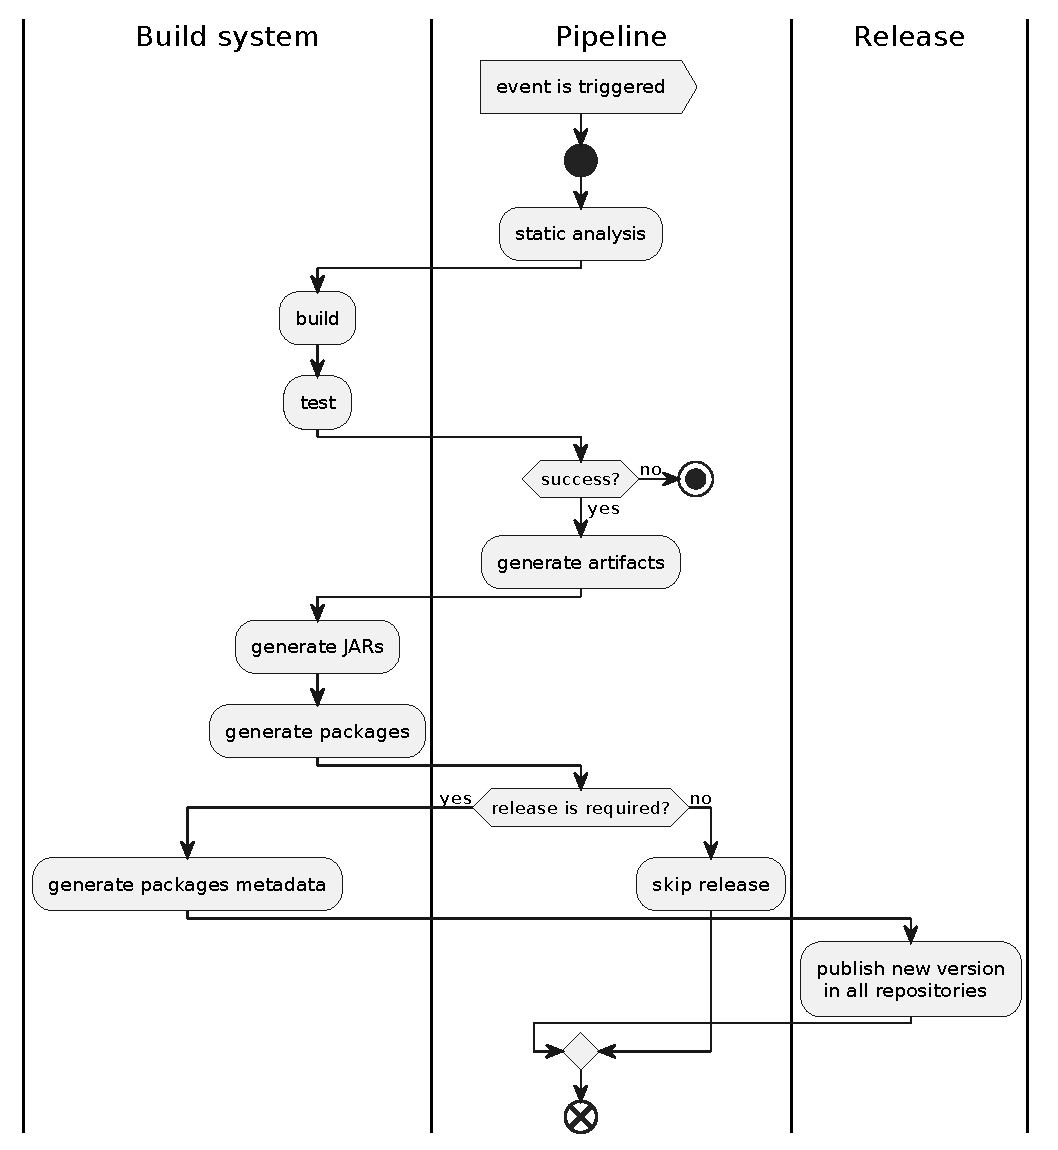
\includegraphics[width=.9\linewidth]{figures/activity-interaction-diagram.pdf}
	\caption{Diagramma di attività raffigurante l'interazione tra i componenti}
	\label{fig:activity-interaction-diagram}
\end{figure}

Nello schema in \cref{fig:activity-interaction-diagram} si fa riferimento ad un generico evento come segnale di avvio della pipeline. Nell'ambito \ac{cicd} l'evento corrisponde spesso alla pubblicazione di nuovo codice nel repository, in modo da generare un processo di integrazione continua del software.

\section{Configurazione del build system}

Il ruolo principale del \textit{build system} è quello di esporre un \textit{task} adibito alla generazione dei pacchetti. Il task dovrà soddisfare i seguenti requisiti:
\begin{itemize}
	\item Deve configurare correttamente le opzioni di \textit{jpackage}, in particolare quelle che mutano nel tempo come la versione.
	\item È necessario stabilire un corretto ordine di esecuzione e albero delle dipendenze per garantire la consistenza del processo.
	\item Deve consentire la dichiarazione di configurazioni differenti a seconda del sistema operativo che esegue il processo.
\end{itemize}

\subsection{Lo strumento jpackage}\label{sec:design-jpackage}
Lo strumento \ac{cli} \textit{jpackage} offre un'interfaccia munita di diverse opzioni per configurare e personalizzare a piacimento i pacchetti in output. Esistono parametri generici, compatibili con tutte le piattaforme, e parametri specifici che vanno a modificare attributi particolari alla tipologia di pacchetto in output scelta. Uno dei motivi che ha portato alla scelta di \textit{jpackage} rispetto ad altri software è la capacità di includere autonomamente una \textit{runtime-image} di Java, ossia una \ac{jre} ridotta di dimensioni all'interno del pacchetto. La combinazione di una \textit{runtime-image} e degli archivi Java (JAR) necessari all'esecuzione dell'applicazione costituiscono l'\textit{application-image}: un pacchetto self-contained che include l'applicazione, assieme una \ac{jvm} e alle librerie necessarie per eseguire quell'applicazione sulla piattaforma di destinazione.

\paragraph{Application image} Alchemist è un progetto modulare e ogni modulo è distribuito in un archivio JAR specifico. Come descritto nella documentazione\footnote{https://alchemistsimulator.github.io/howtos/preparation/jar/index.html} il software predispone due modalità di utilizzo stand-alone attraverso l'esecuzione degli archivi Java. La prima modalità consiste nell'inclusione dei singoli moduli richiesti come \textit{classpath} del processo di esecuzione. La seconda modalità sfrutta l'archivio denominato ``full", ossia un \textit{fat-jar} contenente tutti i moduli e tutte le dipendenze necessarie all'esecuzione del software in tutte le sue parti. In ottica di ridurre le dimensioni del pacchetto e velocizzare il processo di impacchettamento, jpackage costruirà l'\textit{application-image} utilizzando quest'ultimo. Il risultato di un'installazione corretta è differente a seconda della piattaforma di destinazione del pacchetto, nella \cref{fig:application-image-folder-structure} è raffigurata l'organizzazione dei file del software installato in un sistema Linux.  

\begin{figure}
	\centering
	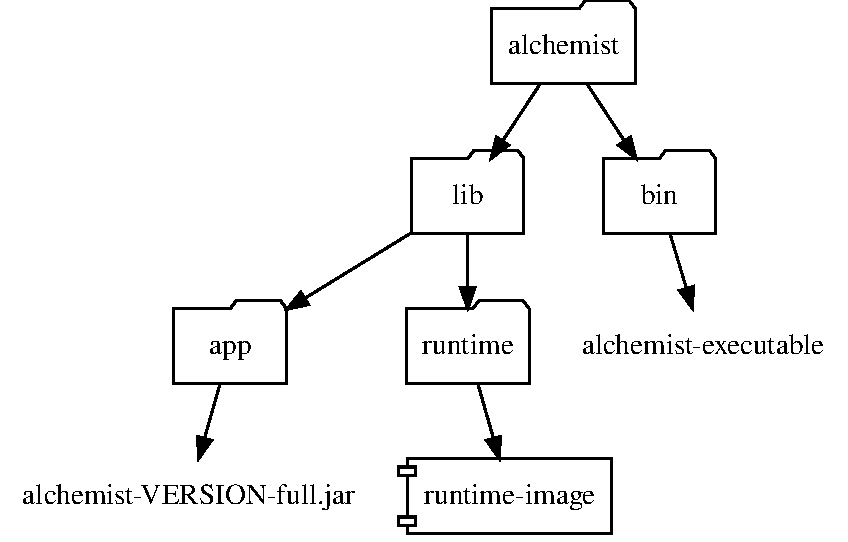
\includegraphics[width=.7\linewidth]{figures/application-image-folder-structure.pdf}
	\caption{Struttura del filesystem dell'\textit{application image} generato da \textit{jpackage} con Linux come piattaforma target}
	\label{fig:application-image-folder-structure}
\end{figure}

\paragraph{Integrazione} Per introdurre jpackage nel build system è necessario un task che funga da \textit{wrapper}: il quale esponga proprietà corrispondenti alle opzioni della \ac{cli} di jpackage. Gradle utilizza una pratica denominata \textit{lazy configuration} che fornisce la dichiarazione delle \textit{lazy properties} vale a dire ``proprietà pigre". Questa caratteristica consente di legare una proprietà a un'altra senza doversi preoccupare dell'ordine di esecuzione. In tale modo non sono necessarie particolari attenzioni nell'assegnazione di proprietà come la versione, la quale viene calcolata da un plugin apposito. 

Il programma jpackage, come illustrato nella sezione \ref{sec:packaging}, non è \textit{cross-platform}, ciò significa che la generazione dei pacchetti deve essere eseguita su una macchina ospitante il sistema operativo di destinazione dei pacchetti richiesti. Per quanto lo strumento cerchi di unificare i diversi ambienti, ogni tipologia di pacchetto specialmente se di piattaforme diverse presenta limiti e caratteristiche differenti. Per questa ragione il task deve prevedere l'utilizzo di parametri differenti a seconda del sistema operativo sottostante.

\subsection{Design finale} Il design ultimo è raffigurato nella \cref{fig:gradle-jpackage-scheme}. 

\begin{figure}[htb]
	\centering
	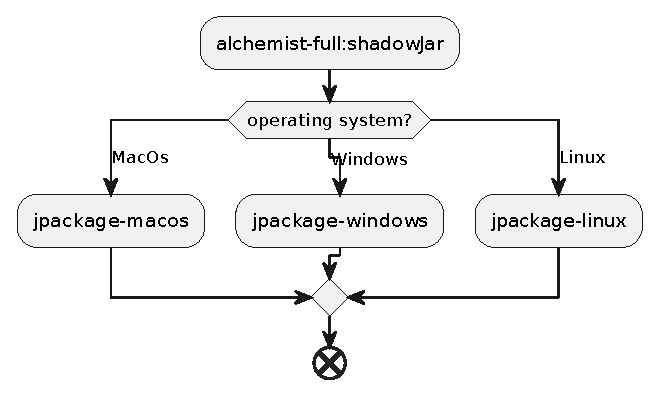
\includegraphics[width=.8\linewidth]{figures/gradle-jpackage-scheme.pdf}
	\caption{Diagramma di attività rappresentante il processo di generazione dei pacchetti}
	\label{fig:gradle-jpackage-scheme}
\end{figure}
\noindent Come discusso nella precedente sezione il design divide la generazione nei tre sistemi operativi target e la sua esecuzione dipende da \texttt{al\-che\-mi\-st\--fu\-ll\-:sha\-dow\-Jar\-}: il task incaricato di generare l'archivio JAR full. In questo modo, quando il task incaricato di generare i pacchetti con jpackage viene invocato, in primo luogo Gradle genera l'archivio JAR necessario a jpackage per costruire un application image valido.

\section{Pipeline}
La pipeline è l'elemento chiave per generare l'automazione dei processi descritti. Alchemist è già provvisto di una pipeline, la quale si occupa di analizzare il codice, verificare i processi di rilascio e in caso sia necessario rilasciare una nuova versione. Il compito del design esplicato in questa sezione è quello di introdurre nuovi step con lo scopo di automatizzare la generazione e distribuzione dei pacchetti generati precedentemente. Le diverse unità di esecuzione o \textit{job} che popolano la pipeline possono essere distinti in base al loro ruolo:
\begin{itemize}
	\item \textbf{Inizializzazione}, tutte le unità incaricate di preparare l'ambiente di esecuzione della pipeline e quindi dei successivi job. 
	\item \textbf{Build e analisi}, i job responsabili di analizzare, compilare ed eseguire i test del codice.
	\item \textbf{Assemblaggio}, le unità di esecuzione responsabili della creazione di artefatti: archivi, pacchetti e documentazione.
	\item \textbf{Test}, job i quali verificano la validità degli artefatti o operazioni come la distribuzione.
	\item \textbf{Rilascio}, i componenti incaricati al rilascio di una nuova versione del software e le relative operazioni accessorie.
\end{itemize}
\begin{figure}[htb]
	\centering
	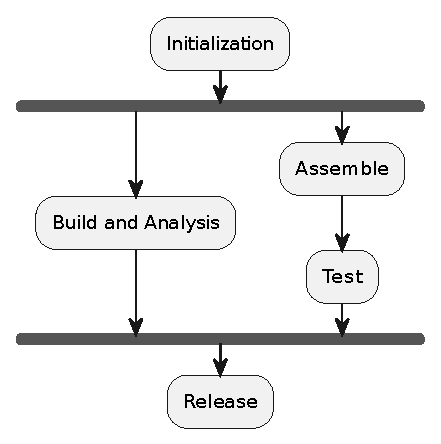
\includegraphics[width=.5\linewidth]{figures/pipeline-roles.pdf}
	\caption{Diagramma di attività illustrante il flusso attraverso i ruoli delineati}
	\label{fig:workflow-roles-summary}
\end{figure}
L'interazione dei processi nella pipeline è raffigurato nella \cref{fig:workflow-roles-summary}. L'\textbf{inizializza\-zio\-ne} trova spazio al primo posto e la sua esecuzione è strettamente necessaria per il proseguimento del flusso. L'\textbf{assemblaggio} e \textbf{build} sono eseguiti parallelamente mentre i \textbf{test} devono inevitabilmente dipendere dalla fase di assemblaggio per poter verificare l'output prodotto da quest'ultimo. Il \textbf{rilascio} infine, richiede che tutte le fasi descritte precedentemente siano eseguite con successo. I ruoli concernenti il lavoro descritto da questo elaborato sono: assemblaggio, test e rilascio.

\subsection{Interazione con il Build System}

Per conseguire gli obiettivi dettati dai ruoli di assemblaggio e test è necessario l'utilizzo del build system. In particolare Alchemist sfrutta lo script \textit{gradle wrapper} per interagire con esso. Il file \textit{gradlew} è uno script che permette di eseguire Gradle senza doverlo installare globalmente: alla prima esecuzione controlla la versione richiesta definita in un file di configurazione, se quest'ultima non è presente allora il wrapper scarica questa e la utilizza per eseguire i task richiesti. I job, le unità di esecuzione della piattaforma GitHub Actions, consentono l'esecuzione di comandi nella \textit{shell} default (oppure una differente) del sistema operativo presente nel runner. In questo modo tramite comandi da shell è possibile eseguire lo script e fornire i task la cui esecuzione è richiesta come argomento di esso.

\paragraph{Test delle funzionalità} Lo \textit{status} di un job indica il risultato dell'esecuzione di esso e può essere: \textit{failure}, \textit{success} oppure \textit{skipped}. Un job è considerato in errore nel caso l'esecuzione di un comando restituisca un valore diverso da 0 e viceversa, perciò non sono necessarie particolari funzionalità per implementare un processo di verifica in quanto il comportamento comune dei comandi rispecchia le regole utilizzate. Lo stato \textit{skipped}, invece, si riferisce ai job non eseguiti secondo condizioni specifiche descritte dallo sviluppatore, è quindi possibile gestire un unico workflow e modificare il suo flusso a seconda dell'evento che ha innescato l'esecuzione. Il comportamento dei job di default all'interno di una pipeline è bloccante per cui il fallimento di uno porta all'interruzione dell'intera pipeline, come raffigurato nel diagramma \cref{fig:activity-diagram-job}.
\begin{figure}[htb]
	\centering
	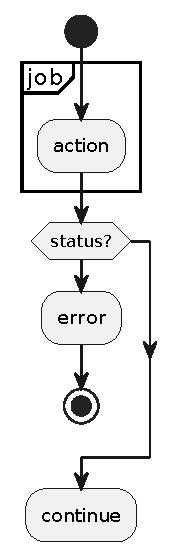
\includegraphics[width=.18\linewidth]{figures/activity-diagram-job.pdf}
	\caption{Diagramma di attività illustrante il comportamento dei job all'interno della pipeline}
	\label{fig:activity-diagram-job}
\end{figure}

Come raffigurato nella \cref{fig:pipeline-activity-diagram}, la pipeline ottenuta inserisce nuovi job adibiti all'assemblaggio e al test dei processi. L'assemblaggio coinvolge tre unità di esecuzione operanti in runner differenti, adibiti alla pacchettizzazione del software nelle tipologie supportate. I job di test racchiudono all'interno le verifiche di validità dei pacchetti generati precedentemente e simula ove possibile la distribuzione del software.
\begin{figure}[htb]
	\centering
	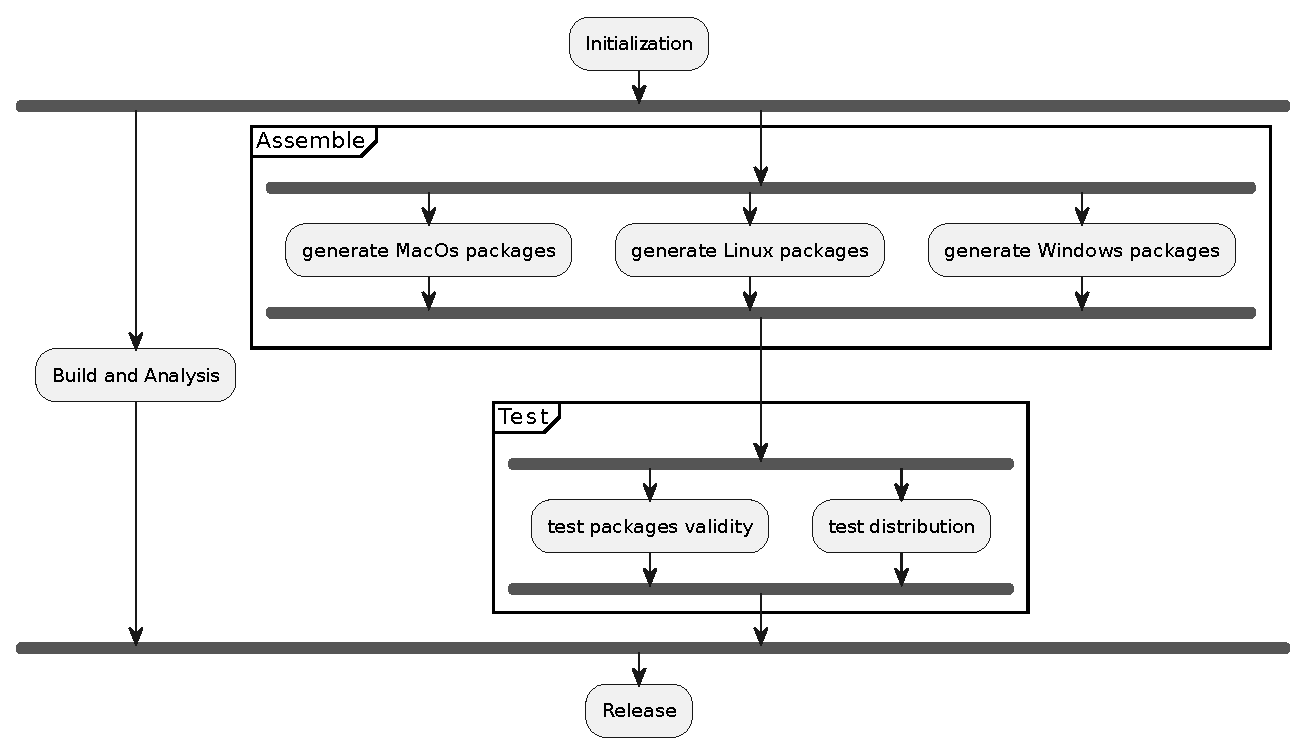
\includegraphics[width=1\linewidth]{figures/pipeline-result.pdf}
	\caption{Diagramma di attività della pipeline risultante}
	\label{fig:pipeline-activity-diagram}
\end{figure}

\newpage
\section{Release}

\subsection{Repository}
Nell'ambito dei package management system, i repository sono i database online da cui i gestori di pacchetti reperiscono gli applicativi. Più genericamente, si intende un qualsiasi archivio online da cui è possibile scaricare software. Ogni repository supporta tipologie di pacchetti e modalità di pubblicazione differenti, le quali sono discusse nella seguente sezione.

\paragraph{AUR} L'Arch User Repository richiede la compilazione di un file PKGBUILD, ossia uno script contenente gli step necessari a scaricare, estrarre, compilare e infine installare il software. Lo script segue uno schema predefinito con parametri obbligatori e altri facoltativi che modificano i meta-dati del pacchetto risultante. Oltre alla presenza di diversi attributi standard, attraverso delle funzioni predefinite è possibile modificare il processo di installazione utilizzando il linguaggio di shell scripting Bash.
Nell'ambito di questo progetto solamente la funzione \textit{package} è necessaria, in quanto il pacchetto sorgente contiene il software pronto per essere eseguito, la funzione dunque si occupa di posizionare i file nel sistema una volta che \texttt{makepkg} ha autonomamente estratto il contenuto del pacchetto di installazione. Per non modificare direttamente il filesystem del computer installante, \texttt{makepkg} crea due directory \textit{pkg} e \textit{src}. All'interno di src, esso estrae il pacchetto con tutto il suo contenuto, mentre pkg simula il filesystem del sistema. La funzione package adibita all'installazione, sposta i file dalla cartella src dentro pkg ricreando il percorso finale che si vuole ottenere sul sistema installante (considerando pkg come root). Una volta generato il pacchetto mediante makepkg, questo può essere installato utilizzando il package manager di riferimento: \textit{pacman}. Esso si occuperà di ricreare la struttura descritta all'interno della directory pkg nel filesystem del sistema installante.

I pacchetti all'interno dell'\ac{aur} consistono in repository \textit{git} contenenti il PKGBUILD e altri file di configurazione opzionali. Il processo di pubblicazione dunque è simile a qualsiasi progetto con un sistema di version control e si articola attraverso quindi: la creazione di un commit con le modifiche al PKGBUILD e la pubblicazione di quest'ultimo.

\paragraph{Winget}\label{chap:winget} Il package manager winget presenta una struttura simile, dove un pacchetto è composto da diversi file manifest che descrivono i metadati del pacchetto nel formato YAML. A differenza del PKGBUILD, non ci sono script e non esistono funzioni, l'intera configurazione è descrittiva e non presenta la possibilità di inserire comandi da eseguire pre o post installazione. I file manifest si distinguono in: manifesto della versione, contenente dettagli identificativi del pacchetto, il manifesto delle impostazioni locali, il quale descrive la configurazione per uno specifico locale, e il manifesto dell'installer, contenente l'URL dove reperire il pacchetto installante e altre informazioni specifiche. Per semplificare il processo di creazione e pubblicazione dei pacchetti, Microsoft prevede l'utilizzo di uno script ``wingetcreate" che guida l'utente nella scelta dei parametri. Questo inoltre si presta a essere utilizzato all'interno di pipeline \ac{cicd} per aggiornare pacchetti già presenti. Il suo utilizzo è quindi necessario per assicurarsi aggiornamenti consistenti, in quanto, lo schema dei manifest può evolversi e cambiare nel tempo. Lo script si occupa autonomamente di aderire ai nuovi schemi, eliminando quindi la necessità per lo sviluppatore di aggiornare il processo di pubblicazione ogni tal volta che una nuova specifica viene pubblicata.

\subsection{Semantic release}
Il processo di \ac{cicd} utilizzato da Alchemist, prevede l'utilizzo di una tecnica chiamata \textit{semantic release}, legata con il più conosciuto concetto di \textit{semantic versioning}. Abbreviato come ``SemVer", esso è uno schema di versionamento standardizzato per determinare le versioni di un software. È stato progettato per rendere intuitivo comprendere le modifiche apportate al software ed il loro impatto riguardo la compatibilità con le versioni precedenti. Lo schema descrive una versione come tre cifre principali separate da punti.
\begin{itemize}
	\item La prima cifra, \textbf{major}, si incrementa quando vengono apportate modifiche sostanziali al software che lo rendono incompatibile con le versioni precedenti.
	\item La seconda, \textbf{minor}, indica l'aggiunta di nuove funzionalità o miglioramenti al software senza eliminare la retro-compatibilità di questo.
	\item La terza cifra, \textbf{patch}, viene incrementata quando una nuova versione risolve bug o problemi di sicurezza.
\end{itemize}
Oltre allo schema principale, SemVer prevede anche la presenza di etichette che stabiliscono se la versione è in fase di sviluppo(alpha, beta) oppure di test.
Attraverso l'utilizzo dei \textit{conventional commits}, il progetto è capace di: stabilire la versione autonomamente, elencare le modifiche tra un rilascio e quello successivo in un \textit{changelog} e decidere quando è necessaria la pubblicazione di una nuova versione. I conventional commits sono un insieme di regole che riguardano i messaggi dei commit, ossia le parti di testo allegate alla modifica del software che lo sviluppatore annette. Le regole stabiliscono una sintassi predefinita che permette di comprendere attraverso la cronologia dei commit le modifiche apportate al software, e inoltre assieme allo schema SemVer permette a tool automatici di calcolare la versione. Nello specifico Alchemist utilizza un plugin di NodeJS capace di analizzare i commit, calcolare la nuova versione e infine pubblicarla. Esso permette attraverso diverse estensioni di modificare il suo comportamento, in particolare: definire i file associati alla nuova versione che saranno disponibili nella release GitHub ed eseguire un comando personalizzato quando avviene la pubblicazione.

\paragraph{Limitazioni}\label{sec:release-limitation} La creazione di una release su GitHub svolta dal plugin determina il rilascio di una nuova versione del software e di conseguenza determina altresì la pubblicazione di essa nei repository pubblici. L'unica modalità per estendere il processo di rilascio e integrare la pubblicazione nei repository winget e \ac{aur} è il comando configurato attraverso il plugin. Questo dettaglio crea delle restrizioni: (i) sul sistema operativo, perché solo un job può prendere in carico il lavoro di rilascio e di conseguenza un solo runner con uno specifico sistema operativo esegue il comando e (ii) l'utilizzo inevitabile di comandi da shell. 